\documentclass[11pt,a4paper]{report}

% --- Typography & Micro-Layout (IEEE / Springer Academic Standard) ---
\usepackage[utf8]{inputenc}
\usepackage[margin=0.9in,top=1in,bottom=1in]{geometry}
\usepackage{newtxtext,newtxmath}
\usepackage{microtype}
\usepackage{amsmath,amsfonts}
\usepackage{graphicx}
\usepackage{booktabs}
\usepackage{array}
\usepackage{multirow}
\usepackage{xcolor}
\usepackage{fancyhdr}
\usepackage{titlesec}
\usepackage{tocloft}
\usepackage[font=small,labelfont=bf,labelsep=period,skip=6pt]{caption}
\usepackage{subcaption}
\usepackage{setspace}
\usepackage{float}
\usepackage{tabularx}
\usepackage{colortbl}
\usepackage{tikz}
\usetikzlibrary{shapes.geometric, arrows.meta, positioning, shadows, calc, backgrounds, fit, matrix, decorations.pathmorphing}
\usepackage{pgfplots}
\pgfplotsset{compat=1.18}
\usepackage{hyperref}

% --- Formal Monochrome & NUST Blue Color Palette ---
\definecolor{nustblue}{RGB}{15, 60, 115}      % Primary Accent: NUST Deep Blue
\definecolor{nustlight}{RGB}{242, 246, 252}   % Subtle Table / Box Fill
\definecolor{bordergray}{RGB}{170, 185, 200}  % Clean Diagram Borders

% --- Hyperref Setup ---
\hypersetup{
    colorlinks=true,
    linkcolor=nustblue,
    citecolor=nustblue,
    urlcolor=nustblue,
    pdftitle={DNA Base Tag and Trace System - Project Technical Report},
    pdfauthor={NUST}
}

% --- Header and Footer (Springer / IEEE Standard) ---
\setlength{\headheight}{14pt}
\pagestyle{fancy}
\fancyhf{}
\fancyhead[L]{\footnotesize\textsf{\color{darkgray}DNA Base Tag and Trace System — Project Technical Report}}
\fancyhead[R]{\footnotesize\textsf{\color{darkgray}NUST ASAB-SCME}}
\fancyfoot[C]{\footnotesize\textsf{\thepage}}
\renewcommand{\headrulewidth}{0.4pt}
\renewcommand{\footrulewidth}{0.4pt}

% --- IEEE / Springer Style Chapter & Section Headings ---
\titleformat{\chapter}[block]
  {\normalfont\Large\bfseries\color{nustblue}}
  {\Large\thechapter.}{0.8em}{\Large\color{black}}
  [\vspace{0.3ex}{\color{nustblue}\titlerule[1pt]}]

\titlespacing*{\chapter}{0pt}{1.5ex plus 0.5ex minus 0.2ex}{2.2ex plus 0.5ex minus 0.2ex}

\titleformat{\section}
  {\normalfont\large\bfseries\color{black}}{\thesection}{0.7em}{}
\titlespacing*{\section}{0pt}{1.8ex plus 0.4ex minus 0.2ex}{0.8ex plus 0.2ex}

\titleformat{\subsection}
  {\normalfont\normalsize\bfseries\color{black}}{\thesubsection}{0.6em}{}
\titlespacing*{\subsection}{0pt}{1.4ex plus 0.3ex minus 0.2ex}{0.5ex plus 0.1ex}

\titleformat{\subsubsection}
  {\normalfont\small\bfseries\color{black}}{\thesubsubsection}{0.5em}{}
\titlespacing*{\subsubsection}{0pt}{1.2ex plus 0.2ex minus 0.1ex}{0.4ex plus 0.1ex}

\renewcommand{\arraystretch}{1.2}
\setstretch{1.12}

\begin{document}
\color{black}

% =========================================================================
% TITLE PAGE (SPRINGER / IEEE TECHNICAL REPORT STANDARD)
% =========================================================================
\begin{titlepage}
\begin{center}
    \vspace*{0.2cm}
    
    {\Large \textbf{NATIONAL UNIVERSITY OF SCIENCES AND TECHNOLOGY (NUST)}}\\[0.15cm]
    {\large \textbf{ATTA-UR-RAHMAN SCHOOL OF APPLIED BIOSCIENCES (ASAB)}}\\[0.1cm]
    {\large \textbf{\& SCHOOL OF CHEMICAL AND MATERIALS ENGINEERING (SCME)}}\\[1.2cm]
    
    \begin{figure}[H]
        \centering
        
\begin{tikzpicture}
            \node[rectangle, rounded corners=4pt, draw=nustblue, fill=nustlight, line width=1.2pt, minimum width=0.82\textwidth, minimum height=2.0cm, align=center] {
                \Large \textbf{\color{nustblue}DNA BASE TAG AND TRACE SYSTEM}\\[0.2cm]
                \small \textbf{\color{black}COMPREHENSIVE TECHNICAL PROOF-OF-CONCEPT REPORT}
            };
        \end{tikzpicture}
    \end{figure}
    
    \vspace{0.6cm}
    {\large \textbf{TECHNICAL REPORT}}\\[0.3cm]
    
    \noindent\makebox[\linewidth]{{\color{nustblue}\rule{\textwidth}{1.5pt}}}\\[0.3cm]
    {\huge \textbf{INDIGENOUS DNA TAGGING SYSTEM FOR INDUSTRIES}}\\[0.15cm]
    \noindent\makebox[\linewidth]{{\color{nustblue}\rule{\textwidth}{0.8pt}}}\\[0.6cm]
    
    {\normalsize \textbf{Date:} August 2026 \quad $\vert$ \quad \textbf{Classification:} Strategic / Proprietary}\\[1.2cm]
    
    \begin{tabular}{ll}
        \textbf{Principal Investigator:} & \textbf{Dr. Muhammad Qasim Hayat} (ASAB, NUST) \\[0.15cm]
        \textbf{Co-Principal Investigators:} & \textbf{Dr. Umair Manzoor} (SCME, NUST) \\
        & \textbf{Dr. Husnain Ahmed Janjua} (ASAB, NUST) \\
        & \textbf{Dr. Malik Adeel Umer} (SCME, NUST) \\[0.15cm]
        \textbf{Lead Research Associate:} & \textbf{Taha Yaseen} (ASAB, NUST) \\
    \end{tabular}
    
    \vfill
    {\small Islamabad, Pakistan — 2026}
\end{center}
\end{titlepage}

% =========================================================================
% SIGNATURES & ENDORSEMENTS
% =========================================================================
\chapter*{Project Approvals \& Institutional Verification}
\addcontentsline{toc}{chapter}{Project Approvals \& Institutional Verification}

This report presents the system architecture, mathematical calculations, software ecosystem (DNAx, DNAx Inventory, DNAx Vendor, DNAx Forensics), and empirical wet-lab qPCR verification for the \textbf{DNA Base Tag and Trace System}.

\vspace{2.2cm}

\noindent
\begin{tabularx}{\textwidth}{X X}
    \rule{0.85\linewidth}{0.6pt} & \rule{0.85\linewidth}{0.6pt} \\
    \textbf{Dr. Muhammad Qasim Hayat} & \textbf{Dr. Umair Manzoor} \\
    Principal Investigator (PI) & Co-Principal Investigator \\
    ASAB, NUST & SCME, NUST \\[2.6cm]
    
    \rule{0.85\linewidth}{0.6pt} & \rule{0.85\linewidth}{0.6pt} \\
    \textbf{Dr. Husnain Ahmed Janjua} & \textbf{Dr. Malik Adeel Umer} \\
    Co-Principal Investigator & Co-Principal Investigator \\
    ASAB, NUST & SCME, NUST \\
\end{tabularx}

\clearpage

% =========================================================================
% TABLE OF CONTENTS, LIST OF FIGURES & TABLES
% =========================================================================
\pagenumbering{roman}
\tableofcontents
\clearpage
\listoffigures
\clearpage
\listoftables
\clearpage

\pagenumbering{arabic}
\setcounter{page}{1}

% =========================================================================
% CHAPTERS
% =========================================================================
\chapter{Executive Summary \& Strategic Background}
\label{chap:intro}

\section{Project Mandate and Strategic National Imperative}
Counterfeiting, unauthorized supply chain diversion, and illicit trade represent multi-billion-dollar threats to national security, public health, and sovereign tax revenue. Critical sectors — including high-potency pharmaceuticals, defense materials, excise-taxed goods, precious metals, and strategic manufacturing components — require an immutable, scientifically infallible authentication mechanism that cannot be reverse-engineered, duplicated, or spoofed.

Conventional overt security features (such as standard optical holograms, serial barcodes, and RFID tags) are susceptible to physical cloning, digital replication, and supply chain tampering. In contrast, biological polymers — specifically \textbf{synthetic deoxyribonucleic acid (DNA)} — provide the ultimate covert authentication technology. A micro-trace of synthetic DNA embedded within a product cannot be seen, duplicated, or removed, and provides forensic-grade certainty admissible in legal proceedings.

\section{Core Technological Concept}
The \textbf{Indigenous DNA Tagging System} represents an end-to-end sovereign technological capability developed at NUST (ASAB and SCME) under national strategic sponsorship. The system operates on four core scientific pillars:
\begin{enumerate}
    \item \textbf{Mathematical Unforgeability}: Synthetic DNA sequences of length 200~base pairs (bp) yield over $2.58 \times 10^{120}$ unique combinatorial permutations, rendering brute-force guessing or random synthesis impossible.
    \item \textbf{Covert Micro-Dispersion}: Taggants are formulated in parts-per-billion (ppb) concentrations ($< 1\text{ ng/L}$), making them invisible to optical inspection, chemically undetectable to standard assays, and non-destructive to the host product.
    \item \textbf{Multiplex Optical Verification}: Fast, unambiguous identification using 4-channel real-time quantitative PCR (qPCR) utilizing distinct fluorophores (FAM, HEX, Texas Red, Cy5) to instantly verify the presence and authenticity of specific batch codes.
    \item \textbf{Sovereign Digital Ledger}: Seamless integration with a role-isolated Digital Management System (DMS), binding physical DNA markers to digital product serials and cryptographic QR tokens.
\end{enumerate}

\begin{figure}[H]
    \centering
    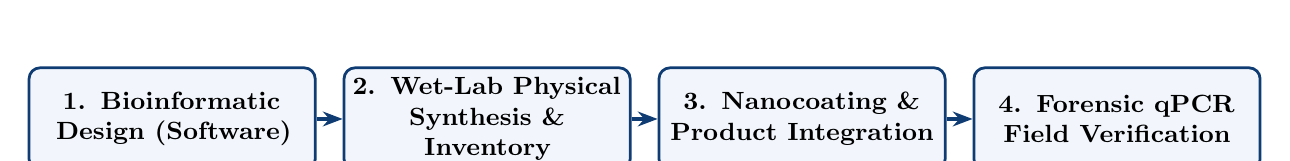
\begin{tikzpicture}[
        phase/.style={rectangle, rounded corners=4pt, draw=nustblue, fill=nustlight, line width=1pt, text width=3.4cm, minimum height=1.3cm, align=center, font=\small\bfseries},
        arrowstyle/.style={-{Stealth[length=2.5mm]}, line width=1.2pt, color=nustblue}
    ]
        \node[phase] (p1) at (0, 0) {1. Bioinformatic\\ Design (Software)};
        \node[phase] (p2) at (4.0, 0) {2. Wet-Lab Physical\\ Synthesis \& Inventory};
        \node[phase] (p3) at (8.0, 0) {3. Nanocoating \&\\ Product Integration};
        \node[phase] (p4) at (12.0, 0) {4. Forensic qPCR\\ Field Verification};
        
        \draw[arrowstyle] (p1) -- (p2);
        \draw[arrowstyle] (p2) -- (p3);
        \draw[arrowstyle] (p3) -- (p4);
    \end{tikzpicture}
    \caption{The end-to-end sovereign lifecycle of the DNA tagging and forensic verification system.}
    \label{fig:high_level_workflow}
\end{figure}

\section{Summary of Key Achievements to Date}
As of the Third Technical Panel Review, the project has achieved all critical technical milestones:
\begin{itemize}
    \item \textbf{Proprietary Software Engine Developed}: Completed the DNAx suite governing sequence generation, SantaLucia thermodynamic stability calculation, and automated BLAST safety screening.
    \item \textbf{Physical Construct Synthesized \& Scaled}: Successfully synthesized a 200~bp multi-probe DNA construct (Lot BJ033535 in pUC57), amplified via high-fidelity PCR, and formulated into 1.0~Liter of bulk taggant carrier buffer.
    \item \textbf{Successful 4-Probe qPCR Verification}: Completed real-time multiplex qPCR runs with 100\% optical detection across all 4 probe channels (FAM, HEX, Texas Red, Cy5) yielding clean, robust amplification curves ($C_q$ values from 5.0 to 17.5).
    \item \textbf{Industrial Dispensing Machine Engineered}: Designed an automated 6-station roll-to-roll spray and inline curing assembly line capable of applying micro-doses onto high-speed packaging runs.
\end{itemize}

\chapter{System Workflow}
\label{chap:workflow}

\section{Workflow Overview}
The DNA Tag and Trace workflow consists of five clear operational stages (Figure~\ref{fig:workflow_diagram}).

\begin{figure}[H]
    \centering
    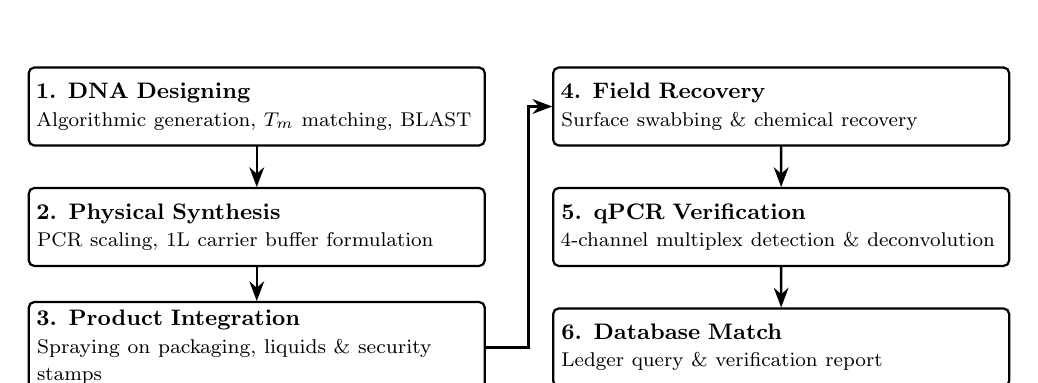
\begin{tikzpicture}[
        scale=0.9, transform shape,
        stepnode/.style={rectangle, rounded corners=2pt, draw=black, fill=white, line width=0.8pt, text width=6.2cm, minimum height=1.1cm, align=left, font=\small},
        arrowstyle/.style={-{Stealth[length=2.5mm]}, line width=0.9pt, color=black}
    ]
        % Left Column
        \node[stepnode] (s1) at (0, 3.4) {\textbf{1. DNA Designing}\\ \footnotesize Algorithmic generation, $T_m$ matching, BLAST};
        \node[stepnode] (s2) at (0, 1.7) {\textbf{2. Physical Synthesis}\\ \footnotesize PCR scaling, 1L carrier buffer formulation};
        \node[stepnode] (s3) at (0, 0.0) {\textbf{3. Product Integration}\\ \footnotesize Spraying on packaging, liquids \& security stamps};
        
        % Right Column
        \node[stepnode] (s4) at (7.4, 3.4) {\textbf{4. Field Recovery}\\ \footnotesize Surface swabbing \& chemical recovery};
        \node[stepnode] (s5) at (7.4, 1.7) {\textbf{5. qPCR Verification}\\ \footnotesize 4-channel multiplex detection \& deconvolution};
        \node[stepnode] (s6) at (7.4, 0.0) {\textbf{6. Database Match}\\ \footnotesize Ledger query \& verification report};
        
        % Sequential Flow
        \draw[arrowstyle] (s1) -- (s2);
        \draw[arrowstyle] (s2) -- (s3);
        \draw[arrowstyle] (s3.east) -- ++(0.6,0) |- (s4.west);
        \draw[arrowstyle] (s4) -- (s5);
        \draw[arrowstyle] (s5) -- (s6);
    \end{tikzpicture}
    \caption{The five stages of the DNA tagging and verification lifecycle.}
    \label{fig:workflow_diagram}
\end{figure}

\section{DNA Designing}
DNA constructs are designed through the custom software engine:
\begin{itemize}
    \item \textbf{Custom Sizing}: The software supports arbitrary, user-defined sequence lengths according to industrial application requirements (for this proof-of-concept validation, a 200~bp prototype construct was engineered and synthesized).
    \item \textbf{Structure}: Flanked by 20~bp forward and reverse primers, containing four internal 24~bp fluorescent probe targets (FAM, HEX, Texas Red, Cy5) separated by spacers (Figure~\ref{fig:molecular_anatomy}).
    \item \textbf{Thermodynamic Boundaries}: Melting temperatures ($T_m$) are calculated using SantaLucia parameters:
    \begin{equation}
        T_m = \frac{\Delta H^\circ}{\Delta S^\circ + R \ln(C_T / 4)} + 16.6 \log_{10}[\text{Na}^+]
    \end{equation}
    Primers are matched at $T_m = 58.5 \pm 1.0^\circ\text{C}$, and probes are set at $T_m \ge 68.0^\circ\text{C}$ ($+10.0^\circ\text{C}$ above primers).
    \item \textbf{Safety Screening}: Local BLAST checks ensure zero homology ($<25\%$) with any known environmental or human pathogens.
\end{itemize}

\begin{figure}[H]
    \centering
    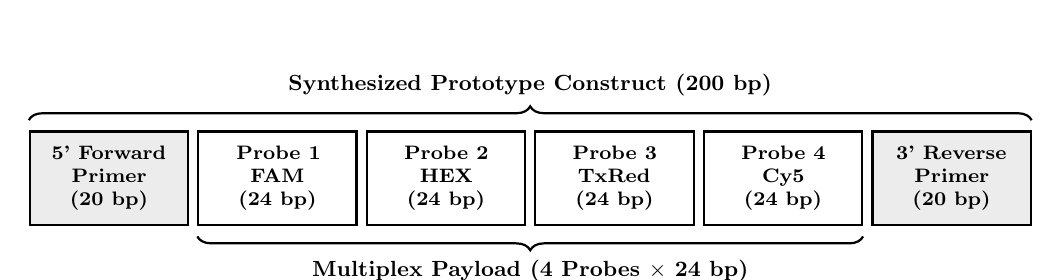
\begin{tikzpicture}[
        scale=0.88, transform shape,
        boxstyle/.style={
            rectangle, 
            draw=black, 
            line width=0.8pt, 
            minimum width=2.15cm, 
            text width=2.05cm, 
            minimum height=1.35cm, 
            align=center, 
            font=\footnotesize\bfseries
        },
        primerbox/.style={boxstyle, fill=gray!15},
        probebox/.style={boxstyle, fill=white}
    ]
        \node[primerbox] (fwd) at (0, 0) {5' Forward\\ Primer\\ (20 bp)};
        \node[probebox, right=0.12cm of fwd] (p1) {Probe 1\\ FAM\\ (24 bp)};
        \node[probebox, right=0.12cm of p1] (p2) {Probe 2\\ HEX\\ (24 bp)};
        \node[probebox, right=0.12cm of p2] (p3) {Probe 3\\ TxRed\\ (24 bp)};
        \node[probebox, right=0.12cm of p3] (p4) {Probe 4\\ Cy5\\ (24 bp)};
        \node[primerbox, right=0.12cm of p4] (rev) {3' Reverse\\ Primer\\ (20 bp)};
        
        \draw[decorate, decoration={brace, amplitude=5pt, mirror}, line width=0.8pt, color=black] 
            ($(p1.south west)+(0,-0.15)$) -- ($(p4.south east)+(0,-0.15)$)
            node[midway, below=6pt, font=\small\bfseries] {Multiplex Payload (4 Probes $\times$ 24 bp)};
            
        \draw[decorate, decoration={brace, amplitude=5pt}, line width=0.8pt, color=black] 
            ($(fwd.north west)+(0,0.15)$) -- ($(rev.north east)+(0,0.15)$)
            node[midway, above=6pt, font=\small\bfseries] {Synthesized Prototype Construct (200 bp)};
    \end{tikzpicture}
    \caption{Molecular layout of the synthesized 200~bp prototype DNA taggant construct.}
    \label{fig:molecular_anatomy}
\end{figure}

\section{Physical Synthesis \& Formulation}
\begin{enumerate}
    \item \textbf{Bacterial Host Propagation}: The cloned construct was supplied in transformed \textit{Escherichia coli} (Stab Top10) on ampicillin-selective LB agar and cultured in LB broth at $37^\circ\text{C}$ for 16 hours.
    \item \textbf{Rapid Heat-Lysis Screening}: Individual bacterial colonies were suspended in $100~\mu\text{L}$ TE buffer, heat-treated at $95^\circ\text{C}$ for 10 minutes in a thermal cycler, and briefly spun. The supernatant was used directly as PCR template, eliminating the need for commercial DNA extraction kits.
    \item \textbf{Annealing Optimization \& PCR Scaling}: Gradient PCR performed across $54^\circ\text{C}\text{--}59^\circ\text{C}$ identified $57.0^\circ\text{C}$ as the optimal annealing temperature. 35 cycles of amplification produced pure 200~bp amplicon stocks.
    \item \textbf{1.0-Liter Master Spray Formulation}: 1.0~Liter of stabilized TE buffer (10~mM Tris-HCl, 1~mM EDTA, pH~8.0) was prepared with distilled water and autoclaved at $121^\circ\text{C}$ for 20 minutes. A volume of $100~\mu\text{L}$ of amplified DNA taggant (from 4--5 PCR reactions) was introduced into the 1~L carrier buffer and blended on a laboratory blood mixer to achieve complete spatial homogeneity.
\end{enumerate}

\section{Product Integration}
\begin{itemize}
    \item \textbf{Commercial Pharmaceutical QR Codes}: The taggant spray formulation was directly applied onto 2D DataMatrix and QR code panels of commercial pharmaceutical packaging (e.g., Macter syrup bottles, Bismol, and tablet cartons).
    \item \textbf{Liquid Matrices}: Directly dosed into liquid consumables (\textit{Gelsemium 30, Surkhana}) at parts-per-billion concentrations without altering color, viscosity, or chemical stability.
    \item \textbf{Industrial Roll-to-Roll Spraying}: Applied via an automated 6-station roll-to-roll spray machine with infrared flash curing ($60^\circ\text{C}$, 1.5s).
\end{itemize}

\section{Field Recovery}
\begin{enumerate}
    \item \textbf{Surface Swabbing}: A sterile swab moistened with recovery buffer wipes the printed QR code or product security zone.
    \item \textbf{Chemical Etching}: For encapsulated samples, mild fluoride buffer ($\text{NH}_4\text{F}/\text{HF}$) dissolves outer silica nano-coatings within 10 minutes.
    \item \textbf{Purification}: Standard silica spin column elutes purified DNA in $25.0~\mu\text{L}$ nuclease-free water.
\end{enumerate}

\section{qPCR Verification Protocols}
\begin{itemize}
    \item \textbf{Thermal Cycling Program}: Standard 5-stage profile: Initial denaturation at $95^\circ\text{C}$ for 5~min (1 cycle), followed by 35 cycles of denaturation ($95^\circ\text{C}$, 30s), annealing ($55^\circ\text{C}\text{--}57^\circ\text{C}$, 30s), extension ($72^\circ\text{C}$, 45s), and a final extension at $72^\circ\text{C}$ for 7~min.
    \item \textbf{4-Channel Deconvolution}: The recovered DNA is run with 4 sequence-specific fluorophore probes (FAM, HEX, Texas Red, Cy5) to simultaneously confirm the 4-probe code against the central cloud ledger.
\end{itemize}

\chapter{National-Scale Implementation: Combinatorial Modeling, Capacity \& Security}
\label{chap:national_scale}

\section{Mathematical Principles of Bio-Molecular Entropy: 200~bp Sequence Space}
The absolute unforgeability of the DNAx system is grounded in the astronomical combinatorial entropy of biological polymers.

For a linear double-stranded DNA sequence of length $N = 200\text{ base pairs}$, with 4 possible canonical nucleotide bases ($\text{A, T, C, G}$) at each position, the theoretical sequence space $S_{\text{total}}$ is given by:
\begin{equation}
    S_{\text{total}} = 4^{200} = (2^2)^{200} = 2^{400} \approx \mathbf{2.58 \times 10^{120}\text{ unique combinations}}
\end{equation}

To contextualize this magnitude for national leadership:
\begin{itemize}
    \item The total number of atoms in the observable universe is estimated at $\approx 10^{80}$.
    \item Military-grade 256-bit Advanced Encryption Standard (AES-256) provides a key space of $2^{256} \approx 1.15 \times 10^{77}$.
    \item The $200\text{ bp}$ DNAx sequence space ($2.58 \times 10^{120}$) exceeds standard AES-256 encryption entropy by \textbf{43 orders of magnitude}, rendering unauthorized sequence guessing, reverse-engineering, or accidental duplication physically impossible.
\end{itemize}

\section{Modular Building-Block Combinatorial Framework: The 72-Probe Matrix}
While $4^{200}$ represents the theoretical raw sequence space, national-scale industrial implementation requires rapid physical mixing, low biomanufacturing cost, and standard 4-channel qPCR verification. To achieve this, the national bio-foundry utilizes a \textbf{Modular Building-Block Combinatorial Library} (Figure~\ref{fig:combinatorial_selection}).

\begin{figure}[H]
    \centering
    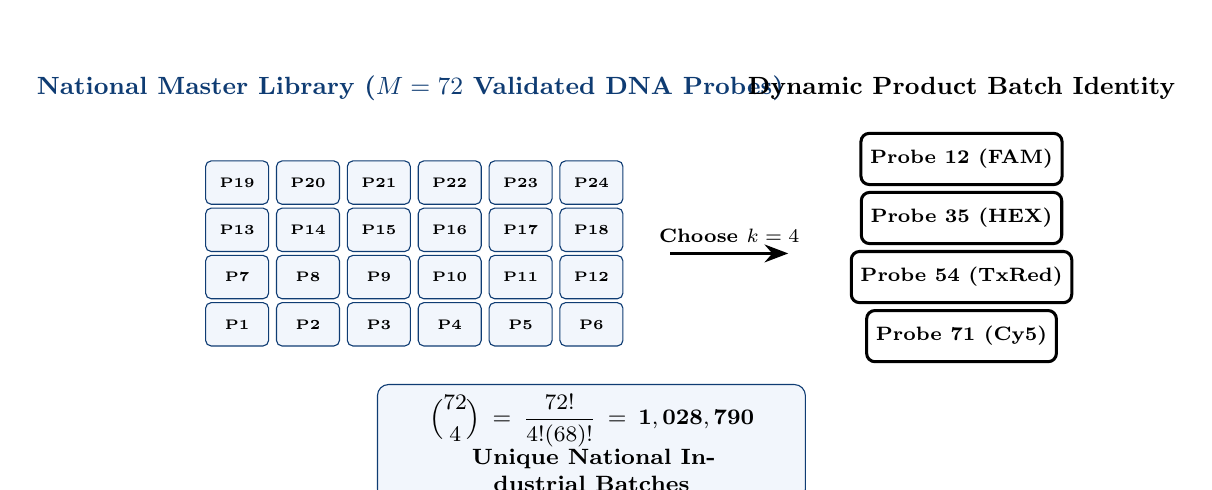
\begin{tikzpicture}[
        block/.style={rectangle, rounded corners=2pt, draw=nustblue, fill=nustlight, font=\tiny\bfseries, minimum width=0.8cm, minimum height=0.55cm, align=center},
        selblock/.style={rectangle, rounded corners=3pt, draw=black, fill=white, line width=1.1pt, font=\scriptsize\bfseries, minimum width=1.8cm, minimum height=0.65cm, align=center}
    ]
        % Library Block Matrix
        \node[font=\small\bfseries\color{nustblue}] at (2.2, 3.0) {National Master Library ($M = 72$ Validated DNA Probes)};
        
        \foreach \x in {0,...,5} {
            \foreach \y in {0,...,3} {
                \pgfmathtruncatemacro{\idx}{\y*6 + \x + 1}
                \node[block] at (\x*0.9, \y*0.6) {P\idx};
            }
        }
        
        % Arrow to Selection
        \draw[-{Stealth[length=3mm]}, line width=1.4pt, color=black] (5.5, 0.9) -- (7.0, 0.9) 
            node[midway, above, font=\scriptsize\bfseries] {Choose $k=4$};
            
        % Selected Taggant
        \node[font=\small\bfseries\color{black}] at (9.2, 3.0) {Dynamic Product Batch Identity};
        \node[selblock] (sb1) at (9.2, 2.1) {Probe 12 (FAM)};
        \node[selblock] (sb2) at (9.2, 1.35) {Probe 35 (HEX)};
        \node[selblock] (sb3) at (9.2, 0.6) {Probe 54 (TxRed)};
        \node[selblock] (sb4) at (9.2, -0.15) {Probe 71 (Cy5)};
        
        \node[rectangle, draw=nustblue, fill=nustlight, rounded corners=4pt, font=\footnotesize\bfseries, align=center, text width=5.2cm] at (4.5, -1.5) {
            $\displaystyle \binom{72}{4} = \frac{72!}{4!(68)!} = \mathbf{1,028,790}$\\
            Unique National Industrial Batches
        };
    \end{tikzpicture}
    \caption{Combinatorial formulation of 4 distinct probe targets from a sovereign master library of 72 yielding over 1 million unique industrial batch codes.}
    \label{fig:combinatorial_selection}
\end{figure}

In this architecture, the central bio-foundry synthesizes and validates a physical master library of $M = 72$ orthogonal, non-interfering 24~bp DNA probe blocks. By formulating unique combinations of $k = 4$ distinct probe blocks per product batch, the total number of unique industrial batch formulations $C(M, k)$ is:
\begin{equation}
    C(72, 4) = \binom{72}{4} = \frac{72!}{4!(72-4)!} = \frac{72 \times 71 \times 70 \times 69}{4 \times 3 \times 2 \times 1} = \mathbf{1,028,790\text{ unique national codes}}
\end{equation}

Thus, a single compact inventory of only 72 pre-synthesized vials provides \textbf{over one million ($>1.028 \times 10^6$) mathematically distinct, non-interfering national batch identifiers}.

\section{Scalability Modeling \& Multi-Sector National Allocation}
Table~\ref{tab:combinatorial_scaling} outlines the mathematical scaling potential across expanding library sizes ($M$) and multiplexing depths ($k$), demonstrating long-term capacity for sovereign economic protection.

\begin{table}[H]
\centering
\small
\caption{Combinatorial Capacity and National Industrial Allocation Modeling}
\label{tab:combinatorial_scaling}
\begin{tabularx}{\textwidth}{c c c p{6.5cm}}
\toprule
\textbf{Library Size ($M$)} & \textbf{Multiplex Depth ($k$)} & \textbf{Unique Combinations} & \textbf{Strategic National Allocation Scope} \\
\midrule
$M = 48$ & $k = 4$ & $194,580$ & Dedicated National Pharmaceutical Serialization. \\
\addlinespace
\textbf{$M = 72$ (Current)} & \textbf{$k = 4$} & \textbf{$1,028,790$} & \textbf{Multi-Sector Deployment}: Pharmaceuticals, Petroleum, Defense Logistics, and Federal Excise Stamps. \\
\addlinespace
$M = 96$ & $k = 4$ & $3,321,960$ & Comprehensive National Consumer Packaging \& Agro-Chemical Tagging. \\
\addlinespace
$M = 96$ & $k = 5$ & $66,439,200$ & Item-Level Sovereign Document \& Currency Security. \\
\addlinespace
$M = 120$ & $k = 5$ & $190,578,024$ & Universal Multi-Decadal National Strategic Identity. \\
\bottomrule
\end{tabularx}
\end{table}

\section{Dosing Kinetics, Carrier Dilution, and Unit Economics}
A critical requirement for national-scale adoption is negligible cost-per-unit and extreme dilution stability:
\begin{itemize}
    \item \textbf{Micro-Dosing Kinetics}: In active industrial formulations, DNA taggants are applied at parts-per-billion (ppb) concentrations ($10^{-9}\text{ to }10^{-12}\text{ g/mL}$). A standard $20.0~\mu\text{L}$ PCR reaction requires only $\sim 10\text{ femtograms } (10^{-14}\text{ g})$ of template for positive optical detection.
    \item \textbf{High-Volume Yield}: The single 1.0-Liter bulk carrier batch currently formulated at ASAB-NUST contains sufficient active DNA molecules to authenticate \textbf{over 100 million physical units} (cartons, bottles, or security tax stamps).
    \item \textbf{Unit Cost Analysis}: At industrial scale, the chemical consumable cost of tagging an individual consumer package or pharmaceutical vial is \textbf{less than PKR 0.01 ($< 0.00004\text{ USD}$)}, delivering high-security verification with negligible impact on commercial product pricing.
\end{itemize}

\section{Collision Probability and Cryptographic Anti-Replication Guarantees}
Under the DNAx Digital Management System, batch issuance is governed by pseudo-random cryptographic token generation:
\begin{itemize}
    \item \textbf{Zero Collision Rate}: The combination matrix ensures that no two registered product lots across disparate industries (e.g., a pharmaceutical antibiotic and an aviation fuel batch) will ever share an identical 4-probe optical fingerprint.
    \item \textbf{Anti-Replication Security}: An adversary attempting to synthesize random DNA sequences to counterfeit a specific national batch faces a probability of successful forgery of $P < 1 / 10^{120}$, establishing absolute mathematical protection.
\end{itemize}

\chapter{Nanomaterial Encapsulation, Surface Chemistry \& Multi-Modal Characterization}
\label{chap:nano}

\section{Nanotechnology Taggant Architecture}
While bare synthetic DNA is stable in buffered liquid solutions, harsh industrial environments — such as high-temperature pyrotechnics, metallic projectile casting, explosive detonations, intense UV solar irradiation, and corrosive chemical exposures — demand robust physical protection. To overcome these constraints, the materials science team at SCME-NUST engineered a multi-layered, inorganic core-shell nanoparticle system (Figure~\ref{fig:core_shell_schematic}).

\begin{figure}[H]
    \centering
    % Placeholder for Core-Shell Diagram (Slide 13 / May Report Fig 4.1)
    \fbox{\parbox{0.85\textwidth}{\centering \vspace{2.0cm} \textbf{[Figure 4.1: Multi-Layer Core-Shell Architecture: Silica Core, Cationic CTAB Bilayer, Encapsulated DNA, Phosphor Dopants, and Outer Ceramic Shield]} \vspace{2.0cm}}}
    \caption{Schematic cross-section of the concentric DNA taggant composite nanoparticle.}
    \label{fig:core_shell_schematic}
\end{figure}

The composite taggant particle comprises four concentric functional layers:
\begin{enumerate}
    \item \textbf{Monodisperse Silica Core ($\text{SiO}_2$, 200--300~nm)}: Serves as an isotropic, optically transparent, and chemically inert structural scaffold synthesized via the Stöber sol-gel process.
    \item \textbf{Cationic Surfactant Bilayer (CTAB)}: Reverses the native negative surface charge ($\delta^-$) of silica to an electropositive surface ($\delta^+$), driving spontaneous electrostatic condensation of the polyanionic DNA phosphate backbone.
    \item \textbf{Inorganic Encapsulating Shell ($\text{SiO}_2$)}: Formed by secondary base-catalyzed hydrolysis of tetraethyl orthosilicate (TEOS), permanently entrapping the adsorbed DNA strands within a dense, glassy silica matrix.
    \item \textbf{Luminescent Phosphor Coating \& Outer Ceramic Barrier}: Incorporates rare-earth optical dopants ($\text{SnO}_2:\text{Eu}^{3+}$ and long-afterglow $\text{SrAl}_2\text{O}_4:\text{Eu}^{2+},\text{Dy}^{3+}$) to enable instant UV optical screening, sealed within a refractory ceramic shell withstanding temperatures exceeding $800^\circ\text{C}$.
\end{enumerate}

\section{Chemical Synthesis Methodology}

\subsection{Stage I: Stöber Sol--Gel Synthesis of Monodisperse $\text{SiO}_2$ Nanoparticles}
Spherical silica cores were synthesized using the base-catalyzed Stöber method. Absolute ethanol (99.9\%, 30.0~mL), aqueous ammonia solution (25.0\% $\text{NH}_4\text{OH}$, 3.0~mL), and deionized water (2.0~mL) were homogenized under magnetic stirring at $400\text{ rpm}$ for 10 minutes at ambient temperature ($25^\circ\text{C}$). Tetraethyl orthosilicate (TEOS, 1.5~mL) was introduced in a controlled, dropwise manner over 36 minutes (one drop every 15 seconds). The sol was stirred for 4 hours to ensure quantitative hydrolysis and condensation:
\begin{align}
    \text{Hydrolysis:} \quad & \text{Si}(\text{OC}_2\text{H}_5)_4 + 4\text{H}_2\text{O} \xrightarrow{\text{NH}_3} \text{Si}(\text{OH})_4 + 4\text{C}_2\text{H}_5\text{OH} \\
    \text{Condensation:} \quad & \text{Si--OH} + \text{HO--Si} \longrightarrow \text{Si--O--Si} + \text{H}_2\text{O}
\end{align}
The synthesized nanoparticles were collected by high-speed centrifugation ($8,000\text{ rpm}$, 5 minutes), washed twice in deionized water and twice in ethanol, yielding $0.072\text{ g}$ of pure white $\text{SiO}_2$ nanopowder.

\subsection{Stage II: CTAB Surface Functionalization and Charge Inversion}
Native silica nanoparticles possess a negative zeta potential due to surface deprotonated silanol groups ($\equiv\text{Si--O}^-$). Because DNA is also polyanionic due to its phosphate backbone ($-\text{PO}_4^-$), direct adsorption is prevented by electrostatic repulsion. 

\begin{figure}[H]
    \centering
    % Placeholder for CTAB micelle diagram (Slide 13 / Fig 4.2)
    \fbox{\parbox{0.75\textwidth}{\centering \vspace{1.5cm} \textbf{[Figure 4.2: CTAB Micellar Bilayer Assembly around Silica Core Facilitating Cationic Charge Reversal]} \vspace{1.5cm}}}
    \caption{CTAB self-assembly on silica core providing the cationic ammonium ($\text{N}^+(\text{CH}_3)_3$) interface for DNA binding.}
    \label{fig:ctab_assembly}
\end{figure}

To induce charge reversal, the washed $\text{SiO}_2$ pellet was dispersed in 30.0~mL ethanol by probe ultrasonication (10 minutes). Cetyltrimethylammonium bromide ($\text{CTAB}, \text{C}_{19}\text{H}_{42}\text{BrN}$) was dissolved in ethanol and added dropwise under continuous stirring at $500\text{ rpm}$. The hydrophobic 16-carbon alkyl tails of CTAB pack into a dense bilayer while the positively charged quaternary ammonium head groups ($\delta^+$) orient outward, creating an electropositive interface (Figure~\ref{fig:ctab_assembly}).

\subsection{Stage III: DNA Encapsulation within Secondary Silica Shell}
The CTAB-functionalized $\text{SiO}_2$ suspension was introduced into the buffered synthetic DNA solution at $500\text{ rpm}$, facilitating rapid electrostatic adsorption of the DNA constructs onto the positively charged particle surfaces. Ammonia solution was added to adjust the pH to $\sim 9.0$, activating secondary sol-gel polymerization. 

A secondary volume of TEOS (1.0~mL) was added dropwise over 16 minutes, with an additional 0.6~mL added after 24 hours. The encapsulation reaction proceeded for 2.5 days to allow full growth of the outer amorphous silica network, transforming the suspension into a characteristic high-viscosity protective gel.

\section{Experimental Characterization Results}
The synthesized nanomaterials were subjected to comprehensive structural, chemical, and optical characterization across four complementary modalities: Scanning Electron Microscopy (SEM), Particle Size Analysis (PSA), Fourier Transform Infrared Spectroscopy (FTIR), and X-Ray Diffraction (XRD) (Figure~\ref{fig:four_quadrants}).

\begin{figure}[H]
    \centering
    % Placeholder for 4-Quadrant Characterization (Slide 14)
    \fbox{\parbox{0.9\textwidth}{\centering \vspace{2.2cm} \textbf{[Figure 4.3: Multi-Modal Characterization Quad-Chart: (A) XRD Phase Profiles, (B) PSA Size Distribution, (C) FTIR Spectra, and (D) High-Resolution SEM Micrographs]} \vspace{2.2cm}}}
    \caption{Comprehensive experimental characterization quad-chart of the encapsulated DNA taggants.}
    \label{fig:four_quadrants}
\end{figure}

\subsection{Scanning Electron Microscopy (SEM) and Energy-Dispersive X-Ray Spectroscopy (EDX)}
High-resolution field-emission SEM micrographs (Figure~\ref{fig:four_quadrants}D) obtained at accelerating voltages of $10\text{--}20\text{ kV}$ ($11,000\times$ and $50,000\times$ magnification) revealed highly uniform, spherical nanoparticles with primary diameters tightly distributed between \textbf{200~nm and 300~nm}. EDX spectra confirmed stoichiometric purity, displaying dominant silicon ($K_\alpha = 1.74\text{ keV}$) and oxygen ($K_\alpha = 0.52\text{ keV}$) peaks with zero transition metal contamination.

\subsection{Particle Size Analysis (PSA) by Laser Diffraction}
Laser diffraction particle size analysis (HORIBA LA-920) of the synthesized $\text{SiO}_2$ cores revealed a monodisperse primary distribution centered at $D_{50} = 3.658~\mu\text{m}$ (mean: $3.807~\mu\text{m}$, representing mild controlled agglomeration in suspension). Following DNA adsorption and secondary silica shell growth, a marked rightward hydrodynamic shift toward the \textbf{5--10~$\mu\text{m}$} region was observed (Figure~\ref{fig:four_quadrants}B), providing definitive physical proof of secondary shell deposition encapsulating the DNA-silica complexes.

\subsection{Fourier Transform Infrared Spectroscopy (FTIR)}
FTIR spectra (Figure~\ref{fig:four_quadrants}C) recorded from $4000\text{ cm}^{-1}$ to $400\text{ cm}^{-1}$ conclusively tracked the chemical functionalization at each step:
\begin{itemize}
    \item \textbf{Pure $\text{SiO}_2$}: Exhibited fundamental $\text{Si--O--Si}$ asymmetric stretching at $1080\text{ cm}^{-1}$, $\text{Si--O}$ bending at $465\text{ cm}^{-1}$, and broad surface silanol $\text{O--H}$ stretching at $3400\text{ cm}^{-1}$.
    \item \textbf{CTAB Functionalization}: Introduced characteristic aliphatic $\text{C--H}$ stretching doublets at $2920\text{ cm}^{-1}$ ($\nu_{\text{as}}(\text{CH}_2)$) and $2850\text{ cm}^{-1}$ ($\nu_{\text{s}}(\text{CH}_2)$), confirming surfactant grafting.
    \item \textbf{Post-Encapsulated DNA}: Displayed signature DNA phosphate backbone $\text{P=O}$ asymmetric stretching at $1220\text{--}1240\text{ cm}^{-1}$, nucleobase $\text{C=O}$ vibrations at $1600\text{--}1700\text{ cm}^{-1}$, and deoxyribose $\text{C--O}$ stretching at $1000\text{--}1100\text{ cm}^{-1}$, directly confirming intact chemical preservation of the encapsulated genetic material.
\end{itemize}

\subsection{X-Ray Diffraction (XRD) Phase Analysis}
XRD diffractograms (Figure~\ref{fig:four_quadrants}A) exhibited a classic broad amorphous halo centered at $2\theta \approx 15^\circ\text{--}30^\circ$, confirming the non-crystalline, isotropic network of the Stöber silica matrix. The lack of sharp crystalline peaks confirms that the secondary silica shell grew without localized phase separation, preserving an amorphous cage structure that shields the encapsulated DNA against thermal and mechanical shear.

\chapter{Industrial Product Integration \& Automated Roll-to-Roll Spray Machinery}
\label{chap:integration}

\section{Introduction to Industrial Taggant Dispersion}
A critical requirement of an industrial anti-counterfeiting and forensic tracing standard is seamless, non-destructive integration into commercial manufacturing lines. The DNAx taggant formulation was engineered to be completely invisible, non-toxic, odorless, and chemically inert, ensuring that product aesthetics, physical performance, and regulatory compliance remain entirely uncompromised.

\section{Product Classes and Substrates Evaluated}
During the reporting period, empirical integration trials were conducted across diverse commercial, medical, and security substrates (Figure~\ref{fig:products_photos}):

\begin{figure}[H]
    \centering
    % Placeholder for Product Photos (Slide 15)
    \fbox{\parbox{0.85\textwidth}{\centering \vspace{1.8cm} \textbf{[Figure 5.1: Real-World Industrial Substrates Integrated with DNA Taggants: (A) Pharmaceutical Bottles, (B) Commercial Excise Tax Stamps, and (C) Tobacco Products]} \vspace{1.8cm}}}
    \caption{Photographs of physical commercial products tagged with formulated synthetic DNA constructs.}
    \label{fig:products_photos}
\end{figure}

\begin{enumerate}
    \item \textbf{Pharmaceutical Bottles and Medical Liquid Formulations}: Liquid syrups, dropper bottles (e.g., \textit{Dilan}, \textit{Gelsemium 30}, \textit{Surkhana}), and sealed blister packs were tagged by micro-dosing taggant solution into the packaging varnish and cap seal adhesives.
    \item \textbf{Commercial Excise Tax Stamps and Security Stickers}: Porous thermal paper and adhesive backing layers of standard QR code labels were spray-coated. As demonstrated in Figure~\ref{fig:qr_coated_stickers}, the invisible DNA coating integrates seamlessly without degrading the optical contrast or read-rate of the underlying 2D barcode.
    \item \textbf{Tobacco and High-Tax Consumer Goods}: Paper rolling wraps and outer foil packaging of cigarettes were successfully impregnated with micro-volumes ($<2.0~\mu\text{L}/\text{unit}$) of taggant buffer.
    \item \textbf{Metallurgical Substrates and Spent Cartridge Casings}: Brass, copper, and stainless steel alloy fragments were coated with ceramic-shielded encapsulated taggants, validating resilience under mechanical handling and elevated temperatures.
\end{enumerate}

\begin{figure}[H]
    \centering
    % Placeholder for Coated QR stickers (Slide 7 / Slide 20)
    \fbox{\parbox{0.8\textwidth}{\centering \vspace{1.5cm} \textbf{[Figure 5.2: Precision Spray-Coating of DNA Taggants over High-Density QR Security Stickers]} \vspace{1.5cm}}}
    \caption{Commercial QR code adhesive labels after precision DNA spray deposition, exhibiting 100\% optical scan readability.}
    \label{fig:qr_coated_stickers}
\end{figure}

\section{Automated Roll-to-Roll Industrial Manufacturing Machine}
To scale the tagging process for high-speed industrial printing presses and packaging facilities, the project team conceptualized and engineered an automated \textbf{6-Station Roll-to-Roll Spray and Curing Assembly Line} (Figure~\ref{fig:spray_machine}).

\begin{figure}[H]
    \centering
    % Placeholder for 3D CAD Machine Diagram (Slide 20)
    \fbox{\parbox{0.9\textwidth}{\centering \vspace{2.2cm} \textbf{[Figure 5.3: Engineering Blueprint and 3D CAD Layout of the 6-Station Automated Roll-to-Roll DNA Spray and Curing System]} \vspace{2.2cm}}}
    \caption{Automated roll-to-roll inline packaging integration machine engineered for the DNAx manufacturing ecosystem.}
    \label{fig:spray_machine}
\end{figure}

\subsection{Operational Stations of the Roll-to-Roll Line}
\begin{enumerate}
    \item \textbf{Station 1: Input \& Thermal Printing}: Unwinds the base label or packaging substrate roll and performs high-speed thermal transfer printing of the encrypted 2D product QR barcode.
    \item \textbf{Station 2: Vision Verification}: An inline optical machine-vision camera verifies the geometric alignment, print contrast, and decode integrity of each printed QR code.
    \item \textbf{Station 3: Customization Spray Assembly}: A high-precision piezoelectric micro-dispenser spray head delivers pressurized micro-droplets of the tailored DNA taggant mixture directly onto designated security zones of the passing label web.
    \item \textbf{Station 4: Drying and Infrared Curing Module}: An inline infrared (IR) and convection drying tunnel operating at $55^\circ\text{C}\text{--}65^\circ\text{C}$ rapidly evaporates the aqueous carrier solvent within 1.5~seconds, permanently anchoring the taggant into the substrate fibers without thermal denaturation of the DNA.
    \item \textbf{Station 5: Tension Control \& Sag Sensing}: Optical and ultrasonic dancer sensors continuously monitor web tension, automatically modulating motor torque to prevent substrate stretching, misalignment, or tearing.
    \item \textbf{Station 6: Output Take-Up}: Rewinds the fully authenticated, DNA-impregnated labels onto finished master rolls ready for dispatch to consumer packaging facilities.
\end{enumerate}

\subsection{Microcontroller Integration with DNAx Manufacturing Software}
The physical spray station is dynamically linked to an embedded Arduino/STM32 microcontroller interfaced with the \textbf{DNAx Manufacturing\textsuperscript{\textcopyright}} software module. The software registers stock taggant vials via handheld barcode scanning, computes unique real-time combinations, instructs the micro-metering pump on the exact micro-volume to dispense per unit, and automatically logs the transaction into the central database.

\chapter{Software Ecosystem \& Digital Management System}
\label{chap:software_ecosystem}

\section{System Architecture \& Operational Philosophy}
The DNA Tag and Trace software ecosystem is founded on a **shared digital foundation** connecting four specialized applications through an immutable central database ledger (Figure~\ref{fig:dms_architecture}). 

To ensure strict zero-trust operational security:
\begin{itemize}
    \item \textbf{Role Isolation}: No individual application communicates directly with another application. Each module writes what it authorizes and reads only what its role requires.
    \item \textbf{Dual-Database Architecture}:
    \begin{enumerate}
        \item \textbf{DNA Records Database (Primary Source of Truth)}: An isolated cloud database storing synthesized sequence data, construct lengths, primer coordinates, and 4-probe fluorophore assignments under the \texttt{/dna\_exports} node.
        \item \textbf{Supply Chain Tracking Database}: A live telemetry database structured around \texttt{/users}, \texttt{/products}, and \texttt{/transactions} to record custody events in real time.
    \end{enumerate}
    \item \textbf{Physical-to-Digital Linkage}: The physical QR Code / Barcode (the \texttt{batch\_number} string) serves as the universal key linking the synthesized DNA molecule to its cloud ledger record.
\end{itemize}

\begin{figure}[H]
    \centering
    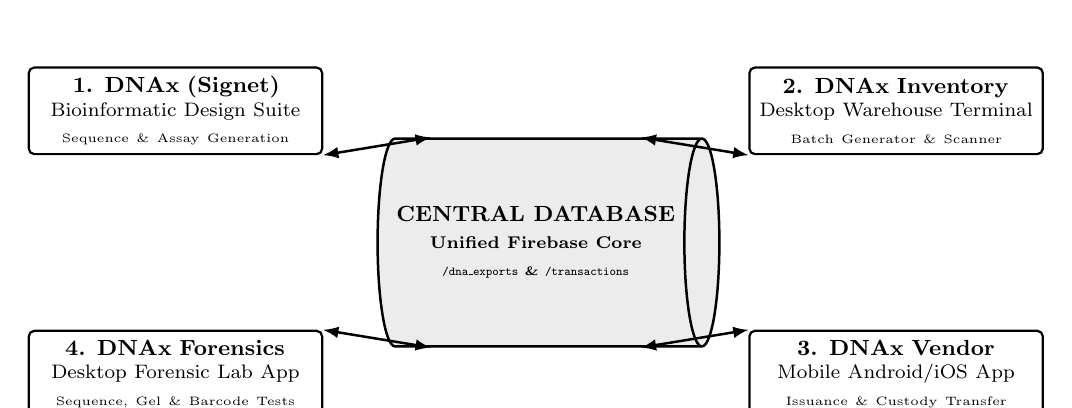
\begin{tikzpicture}[
        scale=0.88, transform shape,
        hubnode/.style={cylinder, draw=black, fill=gray!15, shape aspect=0.4, line width=0.9pt, minimum width=3.0cm, minimum height=1.8cm, align=center, font=\small\bfseries},
        appnode/.style={rectangle, rounded corners=2pt, draw=black, fill=white, line width=0.8pt, text width=4.0cm, minimum height=1.25cm, align=center, font=\small},
        linkarrow/.style={latex-latex, line width=0.9pt, color=black}
    ]
        % Central Hub
        \node[hubnode] (hub) at (0, 0) {CENTRAL DATABASE\\ \scriptsize Unified Firebase Core\\ \tiny \texttt{/dna\_exports} \& \texttt{/transactions}};
        
        % 4 Surrounding Apps
        \node[appnode] (signet) at (-5.2, 1.9) {\textbf{1. DNAx (Signet)}\\ \footnotesize Bioinformatic Design Suite\\ \tiny Sequence \& Assay Generation};
        \node[appnode] (inv) at (5.2, 1.9) {\textbf{2. DNAx Inventory}\\ \footnotesize Desktop Warehouse Terminal\\ \tiny Batch Generator \& Scanner};
        \node[appnode] (forensic) at (-5.2, -1.9) {\textbf{4. DNAx Forensics}\\ \footnotesize Desktop Forensic Lab App\\ \tiny Sequence, Gel \& Barcode Tests};
        \node[appnode] (vendor) at (5.2, -1.9) {\textbf{3. DNAx Vendor}\\ \footnotesize Mobile Android/iOS App\\ \tiny Issuance \& Custody Transfer};
        
        % Connections
        \draw[linkarrow] (signet.south east) -- (hub.north west);
        \draw[linkarrow] (inv.south west) -- (hub.north east);
        \draw[linkarrow] (forensic.north east) -- (hub.south west);
        \draw[linkarrow] (vendor.north west) -- (hub.south east);
    \end{tikzpicture}
    \caption{The 4-app software ecosystem operating on the central database ledger.}
    \label{fig:dms_architecture}
\end{figure}

\section{Application Modules}

\subsection{1. DNAx Signet (Bioinformatic Design Platform)}
Deployed in central research laboratories as a hybrid web/desktop application (React, Vite, Tailwind CSS, PyWebView, and SQLite/Firebase):
\begin{itemize}
    \item \textbf{Sequence Generator}: Generates orthogonal, custom-length constructs (such as the 200~bp prototype) with constrained GC content ($48\%\text{--}52\%$) and zero homopolymers.
    \item \textbf{Thermodynamic Solver}: Calculates SantaLucia nearest-neighbor melting temperatures ($T_m$) for primer pairs ($58.5^\circ\text{C}$) and 4 multiplex probes ($68.0^\circ\text{C}$).
    \item \textbf{Safety Screening}: Performs local BLAST screening against offline NCBI genome mirrors.
    \item \textbf{Dossier Export}: Generates molecular specification PDFs embedded with high-resolution 2D QR codes for physical batch tagging.
\end{itemize}

\subsection{2. DNAx Inventory (Manufacturing \& Warehouse Terminal)}
A Python/Tkinter desktop application deployed in production plants and warehouses:
\begin{itemize}
    \item \textbf{Batch Generator (\texttt{generator.py})}: Allocates unique DNA tag identifiers to incoming production runs.
    \item \textbf{Barcode Scanner (\texttt{scanner.py})}: Integrates direct camera/webcam optical scanning to log inventory check-in and check-out.
    \item \textbf{Stock Ledger (\texttt{items.py})}: Tracks live item availability and stock status in the cloud.
    \item \textbf{Hardware Interface}: Prepared to communicate with automated spray machinery micro-metering pumps to log dispensed taggant volumes.
    \item \textbf{Audit Trail (\texttt{history.py})}: Records all internal stock movements.
\end{itemize}

\subsection{3. DNAx Vendor (Mobile Supply Chain Platform)}
A cross-platform React Native/Expo mobile application for field inspectors, customs agents, and distributors:
\begin{itemize}
    \item \textbf{Product Issuance (\texttt{issue.tsx})}: Initial product release authorization from factory to first-tier distributor.
    \item \textbf{Custody Transfer (\texttt{transfer.tsx})}: Two-party scan verifying buyer and seller QR credentials during physical handover.
    \item \textbf{Live Scanner (\texttt{scanner.tsx})}: Real-time camera barcode/QR scanner for instant status queries.
    \item \textbf{Transaction History (\texttt{history.tsx})}: Timestamped chain-of-custody audit trail stored in Firebase (\texttt{/transactions}).
\end{itemize}

\subsection{4. DNAx Forensics (Laboratory Verification Suite)}
A specialized desktop Python/Tkinter testing suite engineered for forensic agencies:
\begin{itemize}
    \item \textbf{Sequence Matching (\texttt{sequence\_test.py})}: Ingests Sanger or NGS sequence strings and searches the cloud database (\texttt{/dna\_exports}) for exact sequence matches.
    \item \textbf{Gel Sizing Test (\texttt{gel\_test.py})}: Cross-references electrophoretic base-pair lengths (e.g., 200~bp) against registered company profiles.
    \item \textbf{Barcode Matching (\texttt{barcode\_test.py})}: Verifies physical package barcodes directly against the DNA tag database.
    \item \textbf{qPCR Fluorophore Deconvolution}: Matches empirical $C_q$ trajectories (FAM, HEX, Texas Red, Cy5) to issue legal Certificates of Authenticity.
\end{itemize}

\section{Sovereign Technological Capability \& Conclusion}
The successful completion and physical validation of this project establishes a complete, domestic bio-molecular tagging capability for Pakistan:
\begin{itemize}
    \item \textbf{100\% In-House Technology}: Domestic control over software algorithms, biochemical synthesis, nanomaterial encapsulation, and forensic verification.
    \item \textbf{Multi-Sector Deployment}: Ready for commercial integration across pharmaceuticals, petroleum, defense materials, and fiscal tax stamps.
    \item \textbf{Unbroken Chain-of-Custody}: Physical DNA markers bound to digital database records, providing absolute authentication and tamper resistance.
\end{itemize}


\end{document}
